\documentclass{article}\usepackage[]{graphicx}\usepackage[]{xcolor}
% maxwidth is the original width if it is less than linewidth
% otherwise use linewidth (to make sure the graphics do not exceed the margin)
\makeatletter
\def\maxwidth{ %
  \ifdim\Gin@nat@width>\linewidth
    \linewidth
  \else
    \Gin@nat@width
  \fi
}
\makeatother

\definecolor{fgcolor}{rgb}{0.345, 0.345, 0.345}
\newcommand{\hlnum}[1]{\textcolor[rgb]{0.686,0.059,0.569}{#1}}%
\newcommand{\hlstr}[1]{\textcolor[rgb]{0.192,0.494,0.8}{#1}}%
\newcommand{\hlcom}[1]{\textcolor[rgb]{0.678,0.584,0.686}{\textit{#1}}}%
\newcommand{\hlopt}[1]{\textcolor[rgb]{0,0,0}{#1}}%
\newcommand{\hlstd}[1]{\textcolor[rgb]{0.345,0.345,0.345}{#1}}%
\newcommand{\hlkwa}[1]{\textcolor[rgb]{0.161,0.373,0.58}{\textbf{#1}}}%
\newcommand{\hlkwb}[1]{\textcolor[rgb]{0.69,0.353,0.396}{#1}}%
\newcommand{\hlkwc}[1]{\textcolor[rgb]{0.333,0.667,0.333}{#1}}%
\newcommand{\hlkwd}[1]{\textcolor[rgb]{0.737,0.353,0.396}{\textbf{#1}}}%
\let\hlipl\hlkwb

\usepackage{framed}
\makeatletter
\newenvironment{kframe}{%
 \def\at@end@of@kframe{}%
 \ifinner\ifhmode%
  \def\at@end@of@kframe{\end{minipage}}%
  \begin{minipage}{\columnwidth}%
 \fi\fi%
 \def\FrameCommand##1{\hskip\@totalleftmargin \hskip-\fboxsep
 \colorbox{shadecolor}{##1}\hskip-\fboxsep
     % There is no \\@totalrightmargin, so:
     \hskip-\linewidth \hskip-\@totalleftmargin \hskip\columnwidth}%
 \MakeFramed {\advance\hsize-\width
   \@totalleftmargin\z@ \linewidth\hsize
   \@setminipage}}%
 {\par\unskip\endMakeFramed%
 \at@end@of@kframe}
\makeatother

\definecolor{shadecolor}{rgb}{.97, .97, .97}
\definecolor{messagecolor}{rgb}{0, 0, 0}
\definecolor{warningcolor}{rgb}{1, 0, 1}
\definecolor{errorcolor}{rgb}{1, 0, 0}
\newenvironment{knitrout}{}{} % an empty environment to be redefined in TeX

\usepackage{alltt}
\usepackage[sc]{mathpazo}
\renewcommand{\sfdefault}{lmss}
\renewcommand{\ttdefault}{lmtt}
\usepackage[T1]{fontenc}
\usepackage{geometry}
\geometry{verbose,tmargin=2.5cm,bmargin=2.5cm,lmargin=2.5cm,rmargin=2.5cm}
\setcounter{secnumdepth}{2}
\setcounter{tocdepth}{2}
\usepackage[unicode=true,pdfusetitle,
 bookmarks=true,bookmarksnumbered=true,bookmarksopen=true,bookmarksopenlevel=2,
 breaklinks=false,pdfborder={0 0 1},backref=false,colorlinks=false]
 {hyperref}
\hypersetup{
 pdfstartview={XYZ null null 1}}

\makeatletter
%%%%%%%%%%%%%%%%%%%%%%%%%%%%%% User specified LaTeX commands.
\renewcommand{\textfraction}{0.05}
\renewcommand{\topfraction}{0.8}
\renewcommand{\bottomfraction}{0.8}
\renewcommand{\floatpagefraction}{0.75}

\makeatother
\IfFileExists{upquote.sty}{\usepackage{upquote}}{}
\begin{document}



\title{}



\maketitle
The results below are generated from an R script.

\begin{knitrout}
\definecolor{shadecolor}{rgb}{0.969, 0.969, 0.969}\color{fgcolor}\begin{kframe}
\begin{alltt}
\hlcom{### packages}

\hlkwd{library}\hlstd{(stargazer)}
\hlkwd{library}\hlstd{(tidyverse)}
\hlkwd{library}\hlstd{(fixest)}
\hlkwd{library}\hlstd{(devtools)}
\hlkwd{library}\hlstd{(gapminder)}
\hlkwd{library}\hlstd{(xtable)}
\hlkwd{source}\hlstd{(}\hlstr{"functions/collect_coefs.R"}\hlstd{)}

\hlcom{# Set your wd here}
\hlkwd{setwd}\hlstd{(}\hlstr{"~/Desktop/predoc/adao_kehre_lorenzoni"}\hlstd{)}

\hlstd{theme_1} \hlkwb{<-} \hlkwd{theme_bw}\hlstd{()} \hlopt{+}
  \hlkwd{theme}\hlstd{(}\hlkwc{axis.line} \hlstd{=} \hlkwd{element_line}\hlstd{(}\hlkwc{colour} \hlstd{=} \hlstr{"black"}\hlstd{),}
        \hlkwc{panel.grid.minor} \hlstd{=} \hlkwd{element_blank}\hlstd{(),}
        \hlkwc{panel.border} \hlstd{=} \hlkwd{element_rect}\hlstd{(}\hlkwc{colour} \hlstd{=} \hlstr{"black"}\hlstd{),}
        \hlkwc{panel.background} \hlstd{=} \hlkwd{element_blank}\hlstd{(),}
        \hlkwc{plot.title} \hlstd{=} \hlkwd{element_text}\hlstd{(}\hlkwc{hjust} \hlstd{=} \hlnum{0.5}\hlstd{),}
        \hlkwc{text} \hlstd{=} \hlkwd{element_text}\hlstd{(}\hlkwc{size} \hlstd{=} \hlnum{16}\hlstd{),}
        \hlkwc{plot.title.position} \hlstd{=} \hlstr{"plot"}\hlstd{)}

\hlcom{### Importing data}
\hlstd{trade} \hlkwb{<-} \hlkwd{read_csv}\hlstd{(}\hlstr{"data/trade.csv"}\hlstd{)}
\end{alltt}


{\ttfamily\noindent\itshape\color{messagecolor}{\#\# Rows: 4450681 Columns: 5\\\#\# -- Column specification ------------------------------------------------------------------\\\#\# Delimiter: "{},"{}\\\#\# chr (1): hs2\\\#\# dbl (4): year, origin, destination, trade\\\#\# \\\#\# i Use `spec()` to retrieve the full column specification for this data.\\\#\# i Specify the column types or set `show\_col\_types = FALSE` to quiet this message.}}\begin{alltt}
\hlstd{gravity} \hlkwb{<-} \hlkwd{read_csv}\hlstd{(}\hlstr{"data/gravity.csv"}\hlstd{)}
\end{alltt}


{\ttfamily\noindent\itshape\color{messagecolor}{\#\# Rows: 366054 Columns: 8\\\#\# -- Column specification ------------------------------------------------------------------\\\#\# Delimiter: "{},"{}\\\#\# dbl (8): year, origin, destination, distance, contiguity, language, colonial, rta\\\#\# \\\#\# i Use `spec()` to retrieve the full column specification for this data.\\\#\# i Specify the column types or set `show\_col\_types = FALSE` to quiet this message.}}\begin{alltt}
\hlcom{### Task 2: Data manipulation}

\hlcom{## a) collapse}

\hlstd{trade_all} \hlkwb{<-} \hlstd{trade} \hlopt
  \hlkwd{group_by}\hlstd{(year, origin, destination)} \hlopt
  \hlkwd{summarize}\hlstd{(}\hlkwc{trade} \hlstd{=} \hlkwd{sum}\hlstd{(trade))}
\end{alltt}


{\ttfamily\noindent\itshape\color{messagecolor}{\#\# `summarise()` has grouped output by 'year', 'origin'. You can override using the\\\#\# `.groups` argument.}}\begin{alltt}
\hlcom{## b) merging}

\hlstd{tr_merged} \hlkwb{<-} \hlstd{trade_all} \hlopt
  \hlkwd{inner_join}\hlstd{(gravity,} \hlcom{# inner join will only keep obs present in both dtasets}
             \hlkwc{by} \hlstd{=} \hlkwd{c}\hlstd{(}\hlstr{"year"}\hlstd{,} \hlstr{"origin"}\hlstd{,} \hlstr{"destination"}\hlstd{))}

\hlcom{## c) descriptive stats}

\hlstd{desc_stat2015} \hlkwb{<-} \hlstd{tr_merged} \hlopt
  \hlkwd{filter}\hlstd{(year} \hlopt{==} \hlnum{2015}\hlstd{)} \hlopt
  \hlkwd{ungroup}\hlstd{()} \hlopt
  \hlkwd{select}\hlstd{(}\hlopt{-}\hlkwd{c}\hlstd{(year, origin, destination))} \hlopt
  \hlkwd{na.omit}\hlstd{()} \hlopt
  \hlkwd{gather}\hlstd{(Variable, value)} \hlopt
  \hlcom{# Summarize by variable}
  \hlkwd{group_by}\hlstd{(Variable)} \hlopt
  \hlcom{# summarise all columns}
  \hlkwd{summarise}\hlstd{(}\hlkwc{N} \hlstd{=} \hlkwd{sum}\hlstd{(}\hlopt{!}\hlkwd{is.na}\hlstd{(value)),}
            \hlkwc{`Mean`} \hlstd{=} \hlkwd{mean}\hlstd{(value),}
            \hlkwc{`Std. Dev.`} \hlstd{=} \hlkwd{sd}\hlstd{(value),}
            \hlkwc{`Median`} \hlstd{=} \hlkwd{median}\hlstd{(value),}
            \hlkwc{`10th Percentile`} \hlstd{=} \hlkwd{quantile}\hlstd{(value,} \hlnum{.1}\hlstd{),}
            \hlkwc{`90th Percentile`} \hlstd{=} \hlkwd{quantile}\hlstd{(value,} \hlnum{.9}\hlstd{))}

\hlcom{# create a latex table}
\hlstd{desc_tab} \hlkwb{<-} \hlkwd{xtable}\hlstd{(desc_stat2015,}
                   \hlkwc{digits} \hlstd{=} \hlnum{2}\hlstd{,}
                   \hlkwc{caption} \hlstd{=} \hlstr{'Summary statistics for year 2015'}\hlstd{)} \hlopt
  \hlkwd{print}\hlstd{(}\hlkwc{type} \hlstd{=} \hlstr{"latex"}\hlstd{,}
        \hlkwc{include.rownames} \hlstd{=} \hlnum{FALSE}\hlstd{,}
        \hlkwc{format.args} \hlstd{=} \hlkwd{list}\hlstd{(}\hlkwc{big.mark} \hlstd{=} \hlstr{","}\hlstd{),}
        \hlkwc{file} \hlstd{=} \hlstr{"tables/sum2015.tex"}\hlstd{)}

\hlcom{### Task 3: Estimation}

\hlcom{## a)}

\hlcom{# select 2015 and add logged variables}
\hlstd{tr_2015} \hlkwb{<-} \hlstd{tr_merged} \hlopt
  \hlkwd{filter}\hlstd{(year} \hlopt{==} \hlnum{2015}\hlstd{)} \hlopt
  \hlkwd{na.omit}\hlstd{()} \hlopt
  \hlkwd{mutate}\hlstd{(}\hlkwc{log_dist} \hlstd{=} \hlkwd{log}\hlstd{(distance),}
         \hlkwc{log_tr} \hlstd{=} \hlkwd{log}\hlstd{(trade))}


\hlcom{# create bins}
\hlstd{nbins} \hlkwb{=} \hlnum{50}

\hlkwd{pdf}\hlstd{(}\hlkwc{file} \hlstd{=} \hlstr{"fig/binplot.pdf"}\hlstd{)}
\hlstd{tr_2015} \hlopt
  \hlcom{# here I just use equally spaced bins for simplicity}
  \hlkwd{mutate}\hlstd{(}\hlkwc{bin} \hlstd{=} \hlkwd{ntile}\hlstd{(log_tr,} \hlkwc{n} \hlstd{= nbins))} \hlopt
  \hlkwd{group_by}\hlstd{(bin)} \hlopt
  \hlcom{# I summarize the variables by taking the mean inside the bins}
  \hlkwd{summarise}\hlstd{(}\hlkwc{log_tr} \hlstd{=} \hlkwd{mean}\hlstd{(log_tr),} \hlkwc{log_dist} \hlstd{=} \hlkwd{mean}\hlstd{(log_dist))} \hlopt
  \hlkwd{ggplot}\hlstd{(}\hlkwd{aes}\hlstd{(}\hlkwc{x} \hlstd{= log_tr,} \hlkwc{y} \hlstd{= log_dist))} \hlopt{+}
  \hlkwd{geom_point}\hlstd{()} \hlopt{+}
  \hlstd{theme_1} \hlopt{+}
  \hlkwd{labs}\hlstd{(}\hlkwc{title} \hlstd{=} \hlkwd{paste0}\hlstd{(}\hlstr{"Distance and trade: binplot, "}\hlstd{, nbins,} \hlstr{" bins"}\hlstd{,} \hlkwc{sep} \hlstd{=} \hlstr{""}\hlstd{),}
       \hlkwc{x} \hlstd{=} \hlstr{"log(trade), bin mean"}\hlstd{,}
       \hlkwc{y} \hlstd{=} \hlstr{"log(distance), bin mean"}\hlstd{)}
\hlkwd{dev.off}\hlstd{()}
\end{alltt}
\begin{verbatim}
## RStudioGD 
##         2
\end{verbatim}
\begin{alltt}
\hlcom{# pearson correlation}
\hlkwd{print}\hlstd{(}\hlkwd{cor.test}\hlstd{(tr_2015}\hlopt{$}\hlstd{log_tr, tr_2015}\hlopt{$}\hlstd{log_dist))}
\end{alltt}
\end{kframe}

{\centering 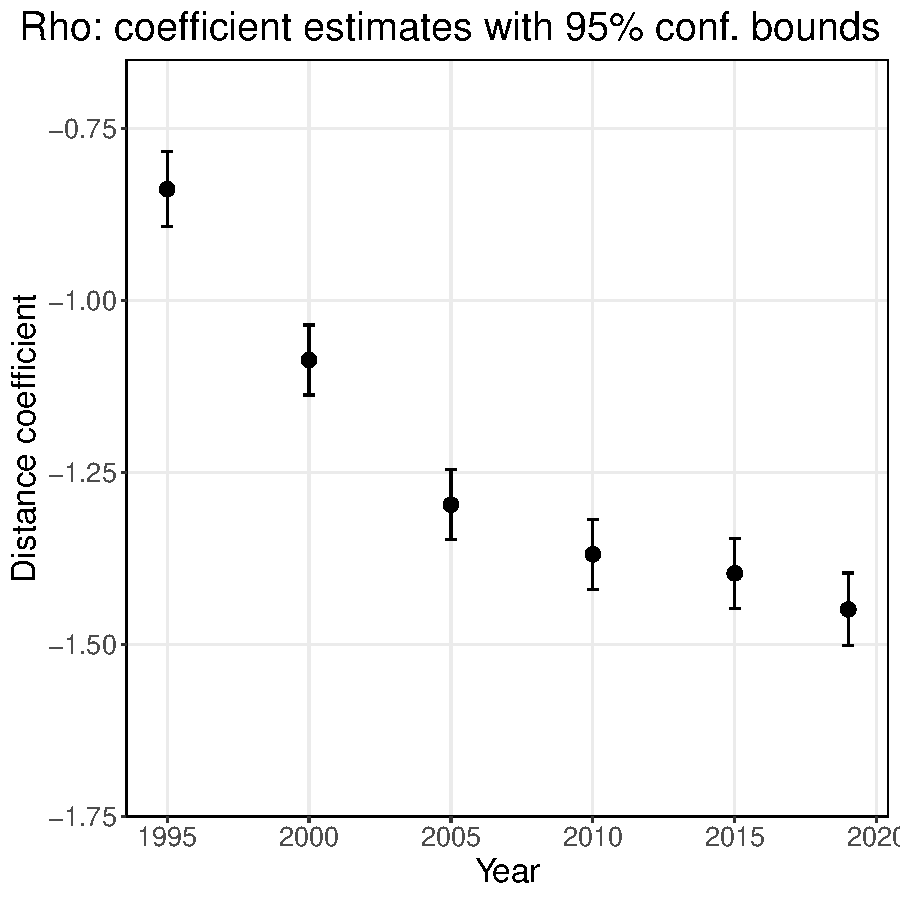
\includegraphics[width=.6\linewidth]{figure/main-Rnwauto-report-1} 

}


\begin{kframe}\begin{verbatim}
## 
## 	Pearson's product-moment correlation
## 
## data:  tr_2015$log_tr and tr_2015$log_dist
## t = -44.021, df = 26936, p-value < 2.2e-16
## alternative hypothesis: true correlation is not equal to 0
## 95 percent confidence interval:
##  -0.2701682 -0.2478874
## sample estimates:
##        cor 
## -0.2590623
\end{verbatim}
\begin{alltt}
\hlcom{## b)}

\hlstd{ols_year} \hlkwb{<-} \hlkwd{feols}\hlstd{(}\hlkwd{log}\hlstd{(trade)} \hlopt{~} \hlkwd{log}\hlstd{(distance),}
                  \hlkwc{data} \hlstd{= tr_merged,} \hlkwc{split} \hlstd{=} \hlopt{~}\hlstd{year)}
\end{alltt}


{\ttfamily\noindent\itshape\color{messagecolor}{\#\# NOTE: 5,460 observations removed because of NA values (RHS: 5,460).}}\begin{alltt}
\hlcom{# collect coefficients manually}
\hlstd{coefs_dst} \hlkwb{<-} \hlkwd{collect_coefs}\hlstd{(}\hlkwc{model} \hlstd{= ols_year,}
                           \hlkwc{variable} \hlstd{=} \hlstr{"log(distance)"}\hlstd{,}
                           \hlkwc{confIntr} \hlstd{=} \hlnum{0.95}\hlstd{)}
\hlstd{coefs_dst} \hlkwb{<-} \hlkwd{as.data.frame}\hlstd{(coefs_dst)} \hlopt
  \hlkwd{mutate_if}\hlstd{(is.character, as.numeric)}


\hlcom{# plot}
\hlkwd{pdf}\hlstd{(}\hlkwc{file} \hlstd{=} \hlstr{"fig/dist_coef_simple.pdf"}\hlstd{)}
\hlstd{coefs_dst} \hlopt
  \hlkwd{ggplot}\hlstd{(}\hlkwd{aes}\hlstd{(}\hlkwc{y} \hlstd{= coef,} \hlkwc{x} \hlstd{= smpl))} \hlopt{+}
  \hlkwd{geom_point}\hlstd{(}\hlkwd{aes}\hlstd{(}\hlkwc{stroke} \hlstd{=} \hlnum{1.5}\hlstd{))} \hlopt{+}
  \hlkwd{geom_errorbar}\hlstd{(}\hlkwd{aes}\hlstd{(}\hlkwc{ymin} \hlstd{= right,} \hlkwc{ymax} \hlstd{= left,} \hlkwc{width} \hlstd{=} \hlnum{.4}\hlstd{))} \hlopt{+}
  \hlstd{theme_1} \hlopt{+}
  \hlkwd{scale_y_continuous}\hlstd{(}\hlkwc{limits} \hlstd{=} \hlkwd{c}\hlstd{(}\hlopt{-}\hlnum{1.7}\hlstd{,} \hlopt{-}\hlnum{0.7}\hlstd{))} \hlopt{+}
  \hlkwd{theme}\hlstd{(}\hlkwc{plot.title} \hlstd{=} \hlkwd{element_text}\hlstd{(}\hlkwc{hjust} \hlstd{=} \hlnum{0.8}\hlstd{),}
        \hlkwc{plot.margin} \hlstd{=} \hlkwd{margin}\hlstd{(}\hlnum{1}\hlstd{,}\hlnum{1}\hlstd{,}\hlnum{1.5}\hlstd{,}\hlnum{1.2}\hlstd{,} \hlstr{"cm"}\hlstd{))}  \hlopt{+}
  \hlkwd{labs}\hlstd{(}\hlkwc{title} \hlstd{=} \hlkwd{TeX}\hlstd{(}\hlstr{"$rho^t$ estimates with 95% conf. bounds"}\hlstd{),}
       \hlkwc{x} \hlstd{=} \hlstr{"Year"}\hlstd{,}
       \hlkwc{y} \hlstd{=} \hlstr{"Distance coefficient"}\hlstd{)}
\hlkwd{dev.off}\hlstd{()}
\end{alltt}
\begin{verbatim}
## RStudioGD 
##         2
\end{verbatim}
\begin{alltt}
\hlcom{## c)}

\hlcom{# since we estimate for each year separately, origin and destination FEs}
\hlcom{# will suffice instead of origin x year and destination x year}
\hlstd{ols_fe} \hlkwb{<-} \hlkwd{feols}\hlstd{(}\hlkwd{log}\hlstd{(trade)} \hlopt{~} \hlkwd{log}\hlstd{(distance)} \hlopt{|} \hlstd{origin} \hlopt{+} \hlstd{destination,}
                \hlkwc{data} \hlstd{= tr_merged,} \hlkwc{split} \hlstd{=} \hlopt{~}\hlstd{year)}
\end{alltt}


{\ttfamily\noindent\itshape\color{messagecolor}{\#\# NOTE: 5,460 observations removed because of NA values (RHS: 5,460).}}\begin{alltt}
\hlcom{# collect the coefficients}
\hlstd{coefs_dst_fe} \hlkwb{<-} \hlkwd{collect_coefs}\hlstd{(}\hlkwc{model} \hlstd{= ols_fe,}
                              \hlkwc{variable} \hlstd{=} \hlstr{"log(distance)"}\hlstd{,}
                              \hlkwc{confIntr} \hlstd{=} \hlnum{0.95}\hlstd{)}
\hlstd{coefs_dst_fe} \hlkwb{<-} \hlkwd{as.data.frame}\hlstd{(coefs_dst_fe)} \hlopt
  \hlkwd{mutate_if}\hlstd{(is.character, as.numeric)}

\hlcom{# plot}
\hlkwd{pdf}\hlstd{(}\hlkwc{file} \hlstd{=} \hlstr{"fig/dist_coef_fe.pdf"}\hlstd{)}
\hlstd{coefs_dst_fe} \hlopt
  \hlkwd{ggplot}\hlstd{(}\hlkwd{aes}\hlstd{(}\hlkwc{y} \hlstd{= coef,} \hlkwc{x} \hlstd{= smpl))} \hlopt{+}
  \hlkwd{geom_point}\hlstd{(}\hlkwd{aes}\hlstd{(}\hlkwc{stroke} \hlstd{=} \hlnum{1.5}\hlstd{))} \hlopt{+}
  \hlkwd{geom_errorbar}\hlstd{(}\hlkwd{aes}\hlstd{(}\hlkwc{ymin} \hlstd{= right,} \hlkwc{ymax} \hlstd{= left,} \hlkwc{width} \hlstd{=} \hlnum{.4}\hlstd{))} \hlopt{+}
  \hlstd{theme_1} \hlopt{+}
  \hlkwd{scale_y_continuous}\hlstd{(}\hlkwc{limits} \hlstd{=} \hlkwd{c}\hlstd{(}\hlopt{-}\hlnum{2}\hlstd{,} \hlopt{-}\hlnum{1.5}\hlstd{))} \hlopt{+}
  \hlkwd{theme}\hlstd{(}\hlkwc{plot.title} \hlstd{=} \hlkwd{element_text}\hlstd{(}\hlkwc{hjust} \hlstd{=} \hlnum{0.8}\hlstd{),}
        \hlkwc{plot.margin} \hlstd{=} \hlkwd{margin}\hlstd{(}\hlnum{1}\hlstd{,} \hlnum{1}\hlstd{,} \hlnum{1.5}\hlstd{,} \hlnum{1.2}\hlstd{,} \hlstr{"cm"}\hlstd{))}  \hlopt{+}
  \hlkwd{labs}\hlstd{(}\hlkwc{title} \hlstd{=} \hlkwd{TeX}\hlstd{(}\hlstr{"$beta^t$ estimates with 95% conf. bounds"}\hlstd{),}
       \hlkwc{x} \hlstd{=} \hlstr{"Year"}\hlstd{,}
       \hlkwc{y} \hlstd{=} \hlstr{"Distance coefficient"}\hlstd{)}
\hlkwd{dev.off}\hlstd{()}
\end{alltt}
\begin{verbatim}
## RStudioGD 
##         2
\end{verbatim}
\begin{alltt}
\hlcom{## d)}


\hlcom{# estimation}
\hlstd{ols_full} \hlkwb{<-} \hlkwd{feols}\hlstd{(}\hlkwd{log}\hlstd{(trade)} \hlopt{~} \hlkwd{log}\hlstd{(distance)} \hlopt{+}
                    \hlstd{contiguity} \hlopt{+} \hlstd{language} \hlopt{+} \hlstd{colonial} \hlopt{+} \hlstd{rta}
                  \hlopt{|} \hlstd{origin} \hlopt{+} \hlstd{destination,}
                  \hlkwc{data} \hlstd{= tr_2015)}
\hlcom{# table}
\hlkwd{etable}\hlstd{(ols_full,} \hlkwc{tex} \hlstd{=} \hlnum{TRUE}\hlstd{,} \hlkwc{file} \hlstd{=} \hlstr{"tables/full.tex"}\hlstd{,} \hlkwc{digits} \hlstd{=} \hlnum{3}\hlstd{,} \hlkwc{replace} \hlstd{= T)}
\end{alltt}
\end{kframe}
\end{knitrout}

The R session information (including the OS info, R version and all
packages used):

\begin{knitrout}
\definecolor{shadecolor}{rgb}{0.969, 0.969, 0.969}\color{fgcolor}\begin{kframe}
\begin{alltt}
\hlkwd{sessionInfo}\hlstd{()}
\end{alltt}
\begin{verbatim}
## R version 4.2.1 (2022-06-23)
## Platform: aarch64-apple-darwin20 (64-bit)
## Running under: macOS Monterey 12.3.1
## 
## Matrix products: default
## LAPACK: /Library/Frameworks/R.framework/Versions/4.2-arm64/Resources/lib/libRlapack.dylib
## 
## locale:
## [1] en_US.UTF-8/en_US.UTF-8/en_US.UTF-8/C/en_US.UTF-8/en_US.UTF-8
## 
## attached base packages:
## [1] stats     graphics  grDevices utils     datasets  methods   base     
## 
## other attached packages:
##  [1] latex2exp_0.9.5 xtable_1.8-4    gapminder_0.3.0 binsreg_0.7     devtools_2.4.5 
##  [6] usethis_2.1.6   fixest_0.11.0   forcats_0.5.2   stringr_1.4.1   dplyr_1.0.9    
## [11] purrr_0.3.4     readr_2.1.2     tidyr_1.2.0     tibble_3.1.8    ggplot2_3.3.6  
## [16] tidyverse_1.3.2 stargazer_5.2.3
## 
## loaded via a namespace (and not attached):
##  [1] googledrive_2.0.0   colorspace_2.0-3    ellipsis_0.3.2      fs_1.5.2           
##  [5] rstudioapi_0.14     farver_2.1.1        MatrixModels_0.5-0  remotes_2.4.2      
##  [9] bit64_4.0.5         fansi_1.0.3         lubridate_1.8.0     xml2_1.3.3         
## [13] splines_4.2.1       cachem_1.0.6        knitr_1.39          pkgload_1.3.0      
## [17] Formula_1.2-4       jsonlite_1.8.0      broom_1.0.0         dbplyr_2.2.1       
## [21] shiny_1.7.2         compiler_4.2.1      httr_1.4.4          backports_1.4.1    
## [25] assertthat_0.2.1    Matrix_1.4-1        fastmap_1.1.0       gargle_1.2.0       
## [29] cli_3.4.1           later_1.3.0         htmltools_0.5.3     quantreg_5.94      
## [33] prettyunits_1.1.1   tools_4.2.1         gtable_0.3.0        glue_1.6.2         
## [37] dreamerr_1.2.3      tinytex_0.41        Rcpp_1.0.9          cellranger_1.1.0   
## [41] vctrs_0.5.0         nlme_3.1-157        xfun_0.32           ps_1.7.1           
## [45] rvest_1.0.3         mime_0.12           miniUI_0.1.1.1      lifecycle_1.0.3    
## [49] googlesheets4_1.0.1 MASS_7.3-57         zoo_1.8-10          scales_1.2.1       
## [53] vroom_1.5.7         hms_1.1.2           promises_1.2.0.1    parallel_4.2.1     
## [57] sandwich_3.0-2      SparseM_1.81        yaml_2.3.5          memoise_2.0.1      
## [61] stringi_1.7.8       highr_0.9           pkgbuild_1.3.1      rlang_1.0.6        
## [65] pkgconfig_2.0.3     matrixStats_0.63.0  evaluate_0.16       lattice_0.20-45    
## [69] htmlwidgets_1.5.4   labeling_0.4.2      bit_4.0.4           processx_3.7.0     
## [73] tidyselect_1.1.2    magrittr_2.0.3      R6_2.5.1            generics_0.1.3     
## [77] profvis_0.3.7       DBI_1.1.3           pillar_1.8.1        haven_2.5.1        
## [81] withr_2.5.0         survival_3.3-1      modelr_0.1.9        crayon_1.5.1       
## [85] utf8_1.2.2          tzdb_0.3.0          rmarkdown_2.15      urlchecker_1.0.1   
## [89] grid_4.2.1          readxl_1.4.1        callr_3.7.2         reprex_2.0.2       
## [93] digest_0.6.29       httpuv_1.6.6        numDeriv_2016.8-1.1 munsell_0.5.0      
## [97] sessioninfo_1.2.2
\end{verbatim}
\begin{alltt}
\hlkwd{Sys.time}\hlstd{()}
\end{alltt}
\begin{verbatim}
## [1] "2022-11-24 16:37:54 +04"
\end{verbatim}
\end{kframe}
\end{knitrout}


\end{document}
